\ifx \globalmark \undefined %% This is default.
	\documentclass[twoside,openright,11pt,a4paper]{report}

%\compiler avec xelatex
%\usepackage[applemac]{inputenc}
\usepackage[T1]{fontenc}
\usepackage[utf8]{inputenc} %latin1 est possible
%\usepackage[latin1]{inputenc} %latin1 est possible
\usepackage[UKenglish]{babel}
\usepackage{lettrine}

%\usepackage[text={13cm,20cm},centering]{geometry}
\usepackage [squaren, Gray, mediumqspace]{SIunits}
\usepackage [top=2cm, bottom=2cm, left=2cm, right=2cm ]{geometry}

\renewcommand{\familydefault}{cmss}
\addto\captionsenglish{ \renewcommand\chaptername{Solutions of Chapte}}

\usepackage{graphicx}
\usepackage{amsmath}
\usepackage{amsfonts}
\usepackage{amssymb}
\usepackage{amsthm}
\usepackage{bm}
\usepackage{color}

\newcommand{\real}{\mathbb{R}}
\newcommand{\mb}{\mathbf}
\newcommand{\bos}{\boldsymbol}

\def \RR {I \! \! R}

\newcommand{\e}{\begin{equation}}  
\newcommand{\ee}{\end{equation}}
\newcommand{\eqn}{\begin{eqnarray}} 
\newcommand{\eeqn}{\end{eqnarray}} 
\newcommand{\eqnn}{\begin{eqnarray*}} 
\newcommand{\eeqnn}{\end{eqnarray*}} 

\newcommand{\bpm}{\begin{pmatrix}}
\newcommand{\epm}{\end{pmatrix}}

%\newcommand{\{\c c}}{\c c}

\newcommand{\bma}{\left(\begin{array}}
\newcommand{\ema}{\end{array}\right)} 
\newcommand{\hh}{\hspace{2mm}}
\newcommand{\hd}{\hspace{5mm}}
\newcommand{\hu}{\hspace{1cm}}
\newcommand{\vv}{\vspace{2mm}}
\newcommand{\vd}{\vspace{5mm}}
\newcommand{\vm}{\vspace{-2mm}}
\newcommand{\teq}{\triangleq}
%\newcommand{\qedb}{\,$\Box$}
\newcommand{\blanc}{$\left. \right.$}
\newcommand{\frts}[2]%
         {\frac{{\textstyle #1}}{{\textstyle #2}}}

\newcommand{\bindex}[3]%
{
\renewcommand{\arraystretch}{0.5}
\begin{array}[t]{c}
#1\\
{\scriptstyle #2}\\
{\scriptstyle #3}
\end{array}
\renewcommand{\arraystretch}{1}
}

\theoremstyle{definition}
\newtheorem{exemple}{{\bf Exemple}}[chapter]
\newtheorem{theoreme}[exemple]{{\bf Th{é}or{è}me}}
\newtheorem{propriete}[exemple]{{\bf Propri{é}t{é}}}
\newtheorem{definition}[exemple]{{\bf D{é}finition}}
\newtheorem{remarque}[exemple]{{\bf Remarque}}
\newtheorem{remarques}[exemple]{{\bf Remarques}}
\newtheorem{lemme}[exemple]{{\bf Lemme}}
\newtheorem{hypothese}[exemple]{{\bf Hypoth{è}se}}
\newtheorem{exercice}{{\bf Exercice}}[chapter]

\newcommand{\xqedhere}[2]{%
 \rlap{\hbox to#1{\hfil\llap{\ensuremath{#2}}}}}

\newcommand{\xqed}[1]{%
 \leavevmode\unskip\penalty9999 \hbox{}\nobreak\hfill
 \quad\hbox{\ensuremath{#1}}}

\newcommand{\gf}{\fg\,\,}

\newcommand{\cata}[1] %
     {\renewcommand{\arraystretch}{0.5}
     \begin{array}[t]{c} \longrightarrow \\ {#1} \end{array}
     \renewcommand{\arraystretch}{1}}

\usepackage[isu]{caption}
%\usepackage[font=small,format=plain,labelfont=bf,up,textfont=it,up]{caption}
\setlength{\captionmargin}{60pt}

\newcommand{\cqfd}
{%
\mbox{}%
\nolinebreak%
\hfill%
\rule{2mm}{2mm}%
\medbreak%
\par%
}

\pagestyle{headings}

\renewcommand{\sectionmark}[1]{%
\markright{\thesection.\ #1}{}}

\renewcommand{\chaptermark}[1]{%
\markboth{\chaptername\ \thechapter.\ #1}{}}

\makeatletter 
\def\@seccntformat#1{\csname the#1\endcsname.\;} 
\makeatother

\title{ {\Huge {\textbf{Modélisation et analyse  \\ \vspace{4mm} des systèmes dynamiques }}} \\ \vspace{4cm} G. Bastin}

%\title{ {\Huge {\textbf{Modelisation et analyse  \\ \vspace{4mm} des systemes dynamiques }}} \\ \vspace{4cm} G. Bastin}


\date{\today}
	\begin{document} %% Crashes if put after (one of the many mysteries of LaTeX?).
\else 
	\documentclass{standalone}
	\begin{document}
\fi

\graphicspath{ {Chapitre1/images/} }

\setcounter{chapter}{0}
\chapter{Systèmes dynamiques et modèles d'état}
\chaptermark{Systèmes dynamiques et modèles d'état}


\lettrine[lines=1]{\bf D}{}ans ce premier chapitre nous donnons tout d'abord la définition de la classe des systèmes dynamiques qui est étudiée dans le livre, ainsi que la terminologie et les notations utilisées, et nous l'illustrons avec divers exemples relevant des sciences de l'ingénieur. Nous expliquons ensuite ce que recouvrent les notions de modélisation et d'analyse des systèmes dynamiques. Le chapitre se termine par une description succincte du contenu des neufs autres chapitres qui constituent le livre.

\section{Définition et exemples} \label{exemple}

Dans ce livre, nous étudierons des systèmes 
dynamiques décrits par des ensembles d'équations différentielles du premier
ordre de la forme
\eqn
\dot x_1&=&f_1(x_1,x_2, \ldots, x_n,u_1,u_2, \ldots u_m), \nonumber\\
\dot x_2&=& f_2(x_1,x_2, \ldots, x_n,u_1,u_2, \ldots u_m), \nonumber\\
\vdots&&\vdots\label{eq:modetn}\\
\dot x_n &=& f_n(x_1,x_2, \ldots, x_n,u_1,u_2, \ldots u_m), \nonumber
\eeqn
où les $f_i$ sont des applications de $\real^{n+m}$ dans $\real$ tandis que les $x_i$ et $u_i$ sont des fonctions scalaires du {\em temps} $t$, qui est une variable indépendante. La quantité $\dot x_i$ représente la dérivée de la variable $x_i$ par rapport au
temps $t$.  Les variables $x_1, x_2, \ldots, x_n$ sont appelées {\em variables
d'état} et contiennent toute l'information nécessaire sur {\em l'état} du
système à l'instant présent pour pouvoir calculer l'évolution de
celui-ci dans le futur, au moyen des équations (\ref{eq:modetn}), étant
données les valeurs futures des variables $u_1, u_2, \ldots, u_m$. 
Celles-ci, appelées {\em entrées} du système, représentent l'influence de l'environnement extérieur sur le système étudié.  On écrit souvent, de manière condensée,  
\e
\dot x = f(x,u)\label{eq:modet}
\ee
où $f$ est une application de $\real^{n+m}$ dans $\real^n$ tandis que $x$ et $u$ sont des fonctions vectorielles du temps. 

Un tel système
d'équations est appelé {\em modèle d'état}. L'objet de ce livre est de traiter
la {\em modélisation}, c'est à dire l'obtention de telles équations dans diverses applications des sciences de l'ingénieur, et {\em l'analyse}, c'est à dire la détermination
des propriétés principales de ces systèmes, déduites des équations.  Nous
commençons par quelques exemples pour illustrer notre propos.
\vv

\begin{exemple}{\bf  Un four de verrerie}

Le premier exemple est un procédé industriel, illustré schématique\-ment
à la figure \ref{fig:fourverre}.  
\begin{figure}[t]
\begin{center}
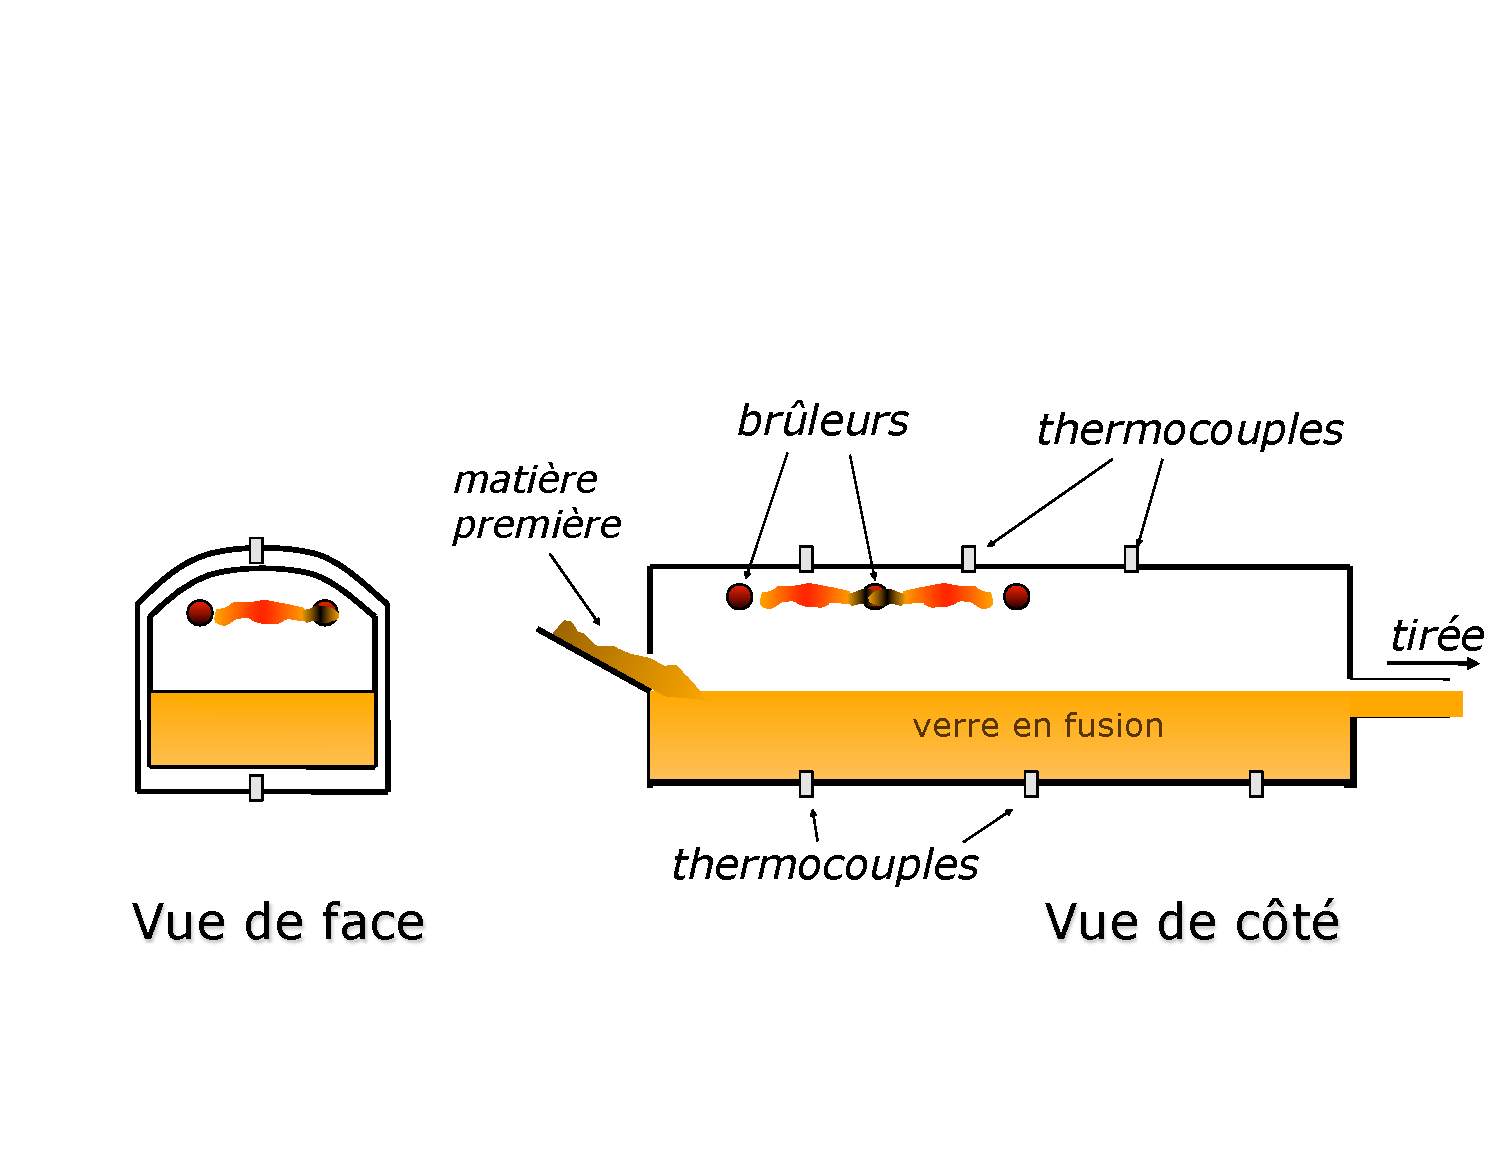
\includegraphics[width=12cm]{fouraverre}
\caption{Four de verrerie}
\label{fig:fourverre}
\end{center}
\end{figure}
Il s'agit d'un four dont les parois sont construites en matériau réfractaire et dans lequel on fait fondre un mélange
de sable, de chaux et d'autres additifs pour obtenir du verre.  Cette fusion est
obtenue par un apport énergétique à l'intérieur du four, provenant par
exemple de brûleurs à gaz disposés au dessus du bain de
verre.  Le verre fondu est extrait du four de manière continue
pour alimenter les machines en aval.  En faisant l'hypothèse que la température du verre est homogène dans
le four et que celui-ci est parfaitement isolé, nous pouvons écrire les deux
équations suivantes, correspondant à un bilan massique et à un bilan énergétique du
procédé. Nous écrivons donc que la variation de masse ou d'énergie, par unité de temps, dans le système considéré est égale à la
somme de  ce qui rentre dans le système, en termes de masse et de chaleur,
diminuée ce qui en sort, toujours durant la même unité de temps:  
\eqn \begin{split}
\frac{dM}{dt} &= P_{in} - P_{out}, \label{eq:bvf} \\
\frac{d}{dt}(CTM) &= Q_{in} + C_{in}T_{in}P_{in}-CTP_{out},
\end{split} \eeqn
avec la signification suivante des variables et paramètres du modèle:\\

$M$ : masse du verre en fusion dans le four (kg),

$T$ : température du verre en fusion dans le four (K),

$T_{in}$ : température de la matière première enfournée (K),

$C$ : chaleur spécifique du verre (J/K$\times$kg),

$C_{in}$: chaleur spécifique de la matière première (J/K$\times$kg),

$Q_{in}$ : quantité de chaleur fournie par unité de temps (J/s),

$P_{in}$ : masse enfournée par unité de temps (kg/s),

$P_{out}$ : masse \og tirée \fg~par unité de temps (kg/s).\\

\noindent Nous avons indiqué des unités pour chacune des grandeurs définies ci-dessus. La cohérence dimensionnelle des équations est la première vérification à effectuer dans un exercice de mise en équation d'un modèle mathématique.

Pour mettre le système d'équations (\ref{eq:bvf}) sous la forme d'un modèle d'état (\ref{eq:modetn}), on définit les variables d'état~:\\

$x_1 \triangleq M$ : masse du verre en fusion (kg),

$x_2 \triangleq C T$ : quantité de chaleur par unité de masse de verre en fusion (J/kg),\\

\noindent et les variables d'entrée~:\\

$u_1 \triangleq P_{in}$ : masse enfournée par unité de temps (kg/s),

$u_2 \triangleq P_{out}$ : masse tirée par unité de temps (kg/s),

$u_3 \triangleq Q_{in}$ : chaleur fournie par unité de temps (J/s).\\

\noindent On obtient alors le modèle d'état~:
\begin{equation} \begin{split} \label{four1}
\dot x_1 &= u_1 - u_2, \\
\dot x_2 &= \dfrac {u_1(\alpha - x_2) + u_3}{x_1},
\end{split} \end{equation}
où le paramètre constant $\alpha = C_{in}T_{in}$ est la quantité de chaleur de la matière enfournée par unité de masse.

On note que d'autres choix des variables d'état et des variables d'entrée sont possibles (voir exercice 1.2). \qed
\end{exemple}  
\vv

\begin{exemple}{\bf  Un réacteur chimique }

\begin{figure}[ht]
\begin{center}
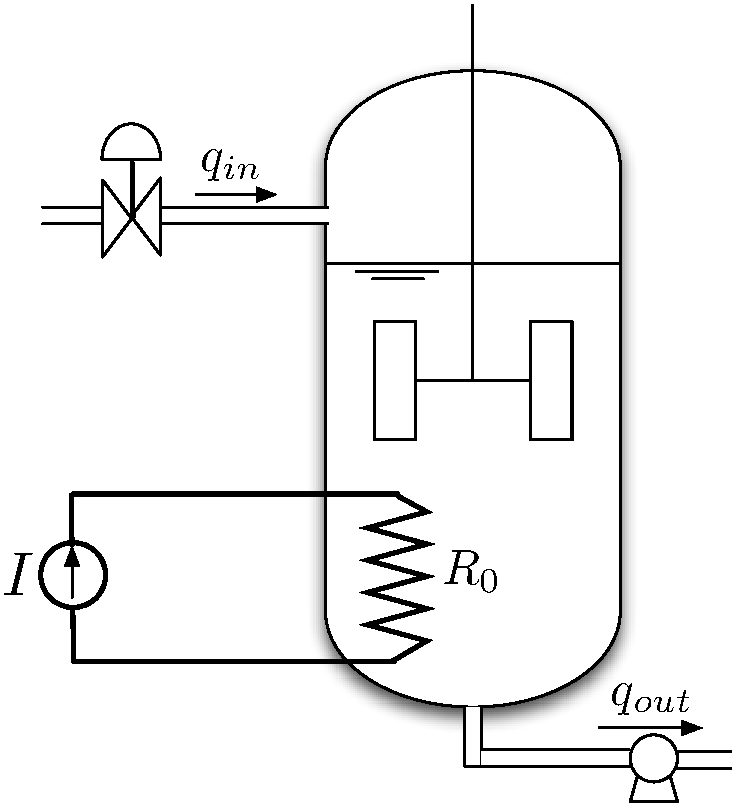
\includegraphics[width=7cm]{reachim}
\caption{Réacteur chimique}
\label{fig:reachim}
\end{center}
\end{figure}
Dans un réacteur chimique (Figure \ref{fig:reachim}), une réaction transformant un réactif A en un produit B se déroule en phase liquide à une certaine température $T$.  Le réacteur est alimenté en réactif
A via une vanne d'alimentation qui introduit le réactif à la concentration
$A_{in}$ avec un débit volumique d'alimentation variable
$q_{in}$ qui est une fonction monotone croissante de l'ouverture de vanne $w$ : $q_{in} = \phi(w)$. Le contenu du réacteur est extrait par une pompe avec un débit de soutirage $q_{out}$. On suppose que la réaction est endothermique et nécessite dès lors un apport calorifique $W$ fourni par une résistance chauffante $R_0$ alimentée par une source de courant variable $I$ comme illustré sur la figure. On suppose en outre que le réacteur est
parfaitement mélangé. La réaction (c.à.d. la transformation du réactif A en
produit B) se passe avec une vitesse de réaction qui obéit à une cinétique du premier ordre, c.à.d. proportionnellement à la quantité de réactif A dans le
réacteur. Le coefficient de proportionnalité est fonction de la température
et vérifie la loi d'Arrhenius, $k(T)=k_0 \exp(-\frac{E}{RT})$.

On décrit l'évolution de ce système en écrivant les équations de bilan volumétrique, massique et thermique:
\begin{equation*} \begin{split} 
&\frac{dV}{dt} = q_{in} - q_{out},\\[0.3em]
&\frac{d}{dt}(AV) = q_{in}A_{in} -q_{out}A-k(T)AV, \\[0.3em]
&\frac{d}{dt}(BV) = -q_{out}B + k(T)AV, \\[0.3em]
&\frac{d}{dt}(CTV) = CT_{in}q_{in}-CTq_{out} - hk(T)AV + R_0I^2,
\end{split} \end{equation*}
avec~:\\

$V$ : volume de liquide dans le réacteur, 

$A$ : concentration en réactif A dans le réacteur,

$B$ : concentration en produit B dans le réacteur,

$k_0$ : constante de vitesse de réaction,

$E$ : énergie d'activation,

$R$ : constante de Boltzmann,

$C$ : chaleur spécifique,

$h$ : enthalpie de réaction.\\

\noindent Les autres notations ont été définies plus haut. En définissant les variables d'état

$x_1 = A$ : concentration en réactif dans le réacteur,

$x_2 = B$ : concentration en produit dans le réacteur,

$x_3 = V$ : volume du milieu réactionnel,

$x_4 = T$ : température du milieu réactionnel,\\

\noindent et les variables d'entrée

$u_1 = w$ : ouverture de vanne,

$u_2 = q_{out}$ : débit de soutirage,

$u_3 = I$ : courant électrique fourni à la résistance chauffante,\\

\noindent on obtient le modèle d'état suivant~:
\begin{equation*} \begin{split} 
\dot x_1 &= \phi(u_1)\dfrac{{\textstyle A_{in} - x_1}}{{\textstyle x_3}} - k(x_4)x_1,\\[0.3em]
\dot x_2 &= - \phi(u_1) \dfrac{x_2}{x_3} + k(x_4)x_1,\\[0.3em]
\dot x_3 &= \phi(u_1) - u_2, \\[0.3em]
\dot x_4 &= \dfrac{{1}}{{x_3}}[\phi(u_1)(T_{in} - x_4) + \dfrac{{R_0}}{{C}}u_3^2] - \dfrac{{h}}{{C}}k(x_4)x_1.
\end{split} \end{equation*}
Les réacteurs {\it continus} et {\it isothermes} constituent un cas particulier intéressant. Il s'agit de réacteurs pour lesquels le volume $V$ et la température $T$ sont maintenus constants par des dispositifs de régulation adéquats. Le modèle d'état est alors réduit aux deux premières équations du modèle ci-dessus~:
\begin{equation} \begin{split} \label{iso}
\dot x_1 &= \dfrac{\phi(u_1)}{{V}} (A_{in} - x_1) - k(T)x_1, \\[0.3em]
\dot x_2 &= - \dfrac{\phi(u_1)}{{V}} x_2 + k(T)x_1.  \xqedhere{4.8cm}{\qed}
\end{split} \end{equation}
\end{exemple}
\vv

\begin{exemple}{\bf Des coccinelles et des pucerons}

Les pucerons sont des insectes ravageurs permanents et redoutables pour les cultures de rosiers. La lutte biologique contre ces ravageurs est une alternative aux traitements par pesticides qui sont de moins en moins efficaces devant les résistances développées par les pucerons. 
\begin{figure}[ht]
\begin{center}
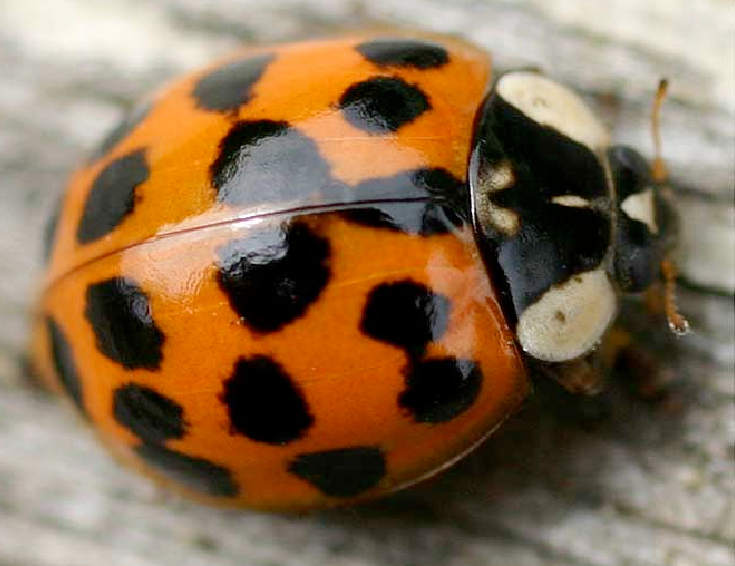
\includegraphics[width=4cm]{cocci}
\caption{Harmonia axyridis}
\label{fig:cocci}
\end{center}
\end{figure}
Les coccinelles {\em Harmonia axyridis} (Fig. \ref{fig:cocci}) sont utilisées dans cette lutte biologique car elles se nourissent de pucerons avec une grande voracité. Elles sont actives dès le printemps, c'est-à-dire dès l'apparition des colonies de pucerons dans les roseraies. Pour augmenter l'efficacité prédatrice des coccinelles, l'Institut Fran\c cais de Recherche Agronomique (INRA) a développé une variété de coccinelles \og sédentaires \gf qui ne volent pas (et ne risquent donc pas de quitter la culture à tra\^ iter).

On souhaite établir un modèle décrivant l'évolution du nombre de pucerons $x_1(t)$ et de coccinelles $x_2(t)$ sous les hypothèses suivantes:
\begin{enumerate}
\item en l'absence de coccinelles, la population de pucerons dispose d'assez de nourriture (les feuilles des rosiers) pour avoir une croissance exponentielle avec un taux spécifique de croissance constant;
\item les coccinelles dévorent d'autant plus de pucerons qu'ils sont nombreux;
\item la prédation par les coccinelles est la seule source de mortalité naturelle des pucerons;
\item les coccinelles ont un taux spécifique constant de mortalité naturelle;
\item le jardinier, qui n'est pas très futé, répand un pesticide qui tue indifférem-ment les pucerons et les coccinelles avec un taux d'épandage variable noté $u(t)$.
\end{enumerate}
Le modèle d'état suivant exprime le bilan du nombre de pucerons et de coccinelles:
\begin{equation} \begin{split}  \label{coc}
\dot x_1 &= ax_1 - bx_1x_2 - cux_1, \\
\dot x_2 &= dx_1x_2 - ex_2 - fux_2. 
\end{split} \end{equation} 
où $a,b,c,d,e,f$ sont des constantes positives. On peut vérifier que chaque terme de ce modèle formalise une des hypothèses ci-dessus. Cette vérification est laissée comme exercice.

Ce type de modèle fut introduit à l'origine par le mathématicien italien V. Volterra qui cherchait à comprendre les fluctuations du rendement de la pêche en mer Adriatique au début du vingtième siècle. Evidemment, il s'agit d'une simplification assez grossière de la réalité. Le modèle ne prend pas en compte de nombreux facteurs qui peuvent influencer l'évolution des populations (conditions climatiques, autres ressources disponibles, autres prédateurs, migration des populations etc ...). Comme l'illustre notre exemple, une application importante de ce type de modèle est la lutte contre les insectes nuisibles dans l'agriculture. Il arrive souvent que la population nuisible soit contr\^olée par l'introduction de prédateurs. Le modèle constitue alors un outil intéressant pour la conception des programmes d'intervention sur le terrain. \qed \\
\end{exemple}


\begin{exemple}{\bf Un moteur à courant continu}

Nous examinons maintenant le dispositif électromécanique illustré à la figure \ref{fig:motdc}.
\begin{figure}[ht]
\begin{center}
\includegraphics[width=6cm]{motdc}
\caption{Moteur à courant continu}
\label{fig:motdc}
\end{center}
\end{figure}
Il s'agit d'un moteur à courant continu qui peut être aussi bien commandé par la tension statorique (ou tension d'excitation) $e$ que par le courant rotorique $I$.
L'équation électrique du circuit statorique est donnée par
\eqnn
e=Ri+L\frac{di}{dt}
\eeqnn
où $R$ et $L$ représentent la résistance et l'inductance du circuit,
$e$ est la tension de commande et $i$ est le courant. Le couple
exercé sur le rotor est donné par $C=\Phi I$ où  $I$ est le courant
rotorique et $\Phi$ est le flux magnétique 
proportionnel au courant d'excitation : $\Phi=Ki$. On obtient donc
\eqnn
C=KiI.
\eeqnn
Il reste à modéliser la partie mécanique de ce système. En notant $\theta$ la
position angulaire du rotor, $J$ son moment d'inertie et  $F$ le coefficient de
frottement visqueux, l'application de la loi de Newton conduit à~:
\eqnn
J\frac{d^2\theta}{dt^2}+F\frac{d\theta}{dt}=C.
\eeqnn

En définissant comme variables d'état $x_1=\theta, x_2=\dot{\theta}, x_3=i$, et
comme entrées $u_1=e$, $u_2=I$, on obtient le modèle d'état suivant:
\begin{equation} \begin{split} \label{motDC}
\dot x_1 &= x_2,  \\[0.3em]
\dot x_2 &= -\frac{F}{J}x_2+\frac{K}{J}x_3u_2, \\[0.3em]
\dot x_3 &= -\frac{R}{L}x_3+\frac{1}{L}u_1. \xqedhere{5cm}{\qed}
\end{split} \end{equation}
\end{exemple}
Les quatre exemples que nous venons de traiter ont pour but de montrer
que l'équation (\ref{eq:modet}) permet effectivement de construire des modèles de systèmes dynamiques dans des domaines variés d'application 
des sciences de l'ingénieur puisque nous avons traité successivement des exemples relevant de la thermodynamique, du génie chimique, de l'écologie et de l'électrotechnique.  Ils permettront aussi de mieux appréhender la terminologie qui est présentée dans la section suivante. 

\section{Terminologie et notations}

Comme les exemples précédents l'ont illustré, nous étudions des {\em systèmes
dynamiques} dont le comportement est décrit par un {\em modèle d'état} formé
d'un ensemble d'équations différentielles écrites sous forme condensée :
\eqn
\dot x = f(x,u). \label{sysdyn}
\eeqn
On considère ce modèle d'état à partir d'un instant initial noté $t_0$. 
L'état $x \in \real^n$ et l'entrée $u \in \real^m$ sont des fonctions vectorielles du
temps que l'on notera parfois $x(t)$ et $u(t)$.  Cependant
l'argument $t$ sera souvent omis sans risque de confusion.

Pour un système donné, l'entrée $u(t)$ est a priori une fonction quelconque du
temps.  On supposera cependant toujours qu'il s'agit d'une fonction {\em continue par morceaux} et {\em
bornée}~: $u(t) \in {\cal U}$ où ${\cal U}$ désigne un ensemble de fonctions continues par morceaux et 
bornées de $\real$ dans $\real^m$.

Pour une valeur donnée de l'état initial $x(t_0) = x_0$ et pour une entrée
$u(t)$ donnée, la solution $x(t) \;\; t \geq t_0$ du système différentiel
(\ref{sysdyn}) est appelée {\em trajectoire} du système.  Parfois, quand ce
sera nécessaire pour la clarté de l'exposé, la trajectoire sera notée
$x(t, x_0, u)$.  Nous supposerons toujours qu'une telle trajectoire existe
à tout instant $t\geq t_0$, est unique et est une fonction continue du temps.
Graphiquement, une trajectoire peut donc être visualisée par une courbe continue dans l'espace $\real^{n+1}$.  La projection de la trajectoire dans
{\em l'espace d'état} $\real^n$ (on dit aussi {\em espace de phase}) est appelée
une {\em orbite} du système.

Lorsque l'entrée $u(t)$ peut être choisie librement dans ${\cal U}$, on dit
que le système $\dot x = f(x,u)$ est un système {\em forcé} ou encore un
système {\em commandé}.  Le qualificatif {\em forcé} est utilisé pour
signifier qu'au départ d'un état initial $x_0$, l'allure de la trajectoire
est en quelque sorte forcée par le choix que l'on a fait d'une entrée $u(t)$. De même, dans un contexte d'automatique, le qualificatif {\em commandé}
signifie que l'état du système peut être piloté dans l'espace d'état par une manipulation appropriée de l'entrée $u(t)$.

Nous serons cependant souvent amenés, dans les chapitres suivants, à nous
intéresser à la solution de l'équation $\dot x = f(x,u)$ lorsque l'entrée est
en réalité une constante fixée a priori : $u(t) = \bar u \;\; \forall t \geq
t_0$.  Dans ce cas, on écrit le modèle d'état sous la forme $\dot x = f(x,
\bar u)$.  Parfois on écrit aussi 
\eqnn
\dot x = f_{\bar u} (x)
\eeqnn
pour exprimer plus clairement que $f$ est une fonction de $x$ seulement,
paramétrée par la constante $\bar u$.  Dans un tel cas, il n'y a évidemment
qu'une seule trajectoire possible évoluant librement au départ d'un état
initial $x_0$.  En fixant d'avance l'entrée à une valeur constante, on se
prive de la possibilité de piloter les trajectoires du système et on dit que
le système est {\em libre} (on dit aussi système {\em autonome} ou système
{\em stationnaire}).  La trajectoire est parfois appelée {réponse libre} du
système.  

Lorsque l'on s'intéresse à la solution de l'équation $\dot x = f(x,u)$ pour
{\em une} entrée $u(t)$ variant au cours du temps mais particulière (par
exemple une sinusoide), on peut tout aussi bien oublier que l'on a
sélectionné cette entrée dans ${\cal U}$ et écrire tout simplement : 
\eqnn
\dot x = f(x,t)
\eeqnn
Un système dynamique représenté de cette manière est appelé système {\em  non
autonome} ou {\em instationnaire}.  

Nous serons parfois amenés à considérer divers cas particuliers du modèle
d'état général (\ref{sysdyn}).  On distinguera notamment~:\\

\noindent \textbf{\textit{Les systèmes affines en l'entrée}}
\eqnn
\dot x = f(x) + \sum^m_{i=1} u_ig_i(x) \triangleq f(x) + G(x)u
\eeqnn
où $f$ et les $g_i$ sont des applications de $\real^n$ dans $\real^n$.
Le modèle d'état \eqref{four1} d'un four de verrerie est de cette forme avec les définitions suivantes~:
\begin{equation*}
f(x) = 0, \hh \hh \hh \hh G(x) = \left(\begin{array}{ccc}
1&-1 & 0 \\[0.3em] (\alpha-x_2)/x_1 & 0 & 1/x_1 \end{array} \right).
\end{equation*}\\

\noindent \textbf{\textit{Les systèmes affines en l'état}}
\eqnn
\dot x = \sum^m_{i=1}x_i a_i(u) + b(u) \triangleq A(u) x + b(u) 
\eeqnn
où $b$ et les $a_i$ sont des applications de $\real^m$ dans $\real^n$. Le modèle d'état d'un réacteur chimique continu isotherme \eqref{iso} est de
cette forme avec les définitions suivantes~:
\begin{equation*} \begin{split}
A(u) &= \left(\begin{array}{cc}
-(\dfrac{\phi(u_1)}{V} +k(T)) & 0 \\[0.3em] k(T) & -\dfrac{ \phi(u_1)}{V}
\end{array} \right),\\[0.5em]
b(u) &=  \left(\begin{array}{c} \dfrac{ \phi(u_1) A_{in}}{V}\\[0.7em] 0
\end{array}\right).
\end{split} \end{equation*}\\

\noindent \textbf{\textit{Les systèmes bilinéaires}}
 
Ce sont des systèmes affines à la fois en l'état et en
l'entrée
\begin{eqnarray*}
\dot x &=& \left ( A_0 + \sum^m_{i=1} u_iA_i \right) x + B_0u, \\[0.3em]
&=& A_0x + (B_0+ \sum^n_{i=1} x_i B_i)u,
\end{eqnarray*}
où les $A_i$ $(i = 0, \ldots, m)$ sont des matrices de dimension $(n
\times n)$ et les $B_i$ $(i = 0, \ldots, n)$ sont des matrices de
dimension $(n \times m)$.  Le modèle d'état d'un moteur à courant continu
(\ref{motDC}) est de cette forme avec les définitions suivantes~:
\begin{equation*} \begin{split}
A_0 &= \left( \begin{array}{ccc}
0 & 1 & 0 \\[0.3em] 0 &-\dfrac{B}{J} & 0\\[0.3em]
0&0& -\dfrac{R}{L}
\end{array}
\right)\;\;\; A_1 = 0
\\
A_2 &= \left( \begin{array}{ccc}
0 & 0 & 0 \\[0.3em] 0 & 0 & \dfrac{K}{J} \\[0.5em]
0 & 0 & 0
\end{array}\right)\hspace*{10mm} B_0 = \left(\begin{array}{cc} 0 & 0 \\[0.3em] 0 & 0 \\[0.3em] \dfrac{1}{L}&0
\end{array} \right).
\end{split} \end{equation*}\\

\noindent \textbf{\textit{Les systèmes linéaires}}
$$
\dot x = Ax +Bu
$$
où $A$ est une matrice de dimension $(n \times n)$ et $B$ est une
matrice de dimension $(n \times m)$.  Si on considère le modèle d'état
du moteur à courant continu en supposant que la source de courant rotorique
est constante ($I$ = constante), on obtient un exemple de système linéaire
avec
\begin{equation*}
A = \left( \begin{array}{ccc}
0 & 1 & 0 \\[0.3em] 0 &-\dfrac{B}{J} & \dfrac{KI}{J}\\[0.9em]
0&0& -\dfrac{R}{L}
\end{array}
\right)\;\;\; B = \left(\begin{array}{cc} 0 & 0 \\[0.3em] 0 & 0 \\[0.3em] \dfrac{1}{L}&0
\end{array} \right).
\end{equation*}
\vv

\section{Modélisation et analyse}

Un système dynamique, tel que nous le concevons dans ce livre, est donc une partie de la réalité {\it concrète} qui nous semble pertinente dans un problème d'ingénierie et que nous choisissons d'isoler par la pensée pour en décrire le comportement en termes mathématiques à l'aide d'un modèle. Nous sommes intéressés en particulier à caractériser quantitativement l'évolution, au cours du temps, de l'{\it état} de ce système. Nous utilisons pour cela des modèles d'état {\it déterministes à paramètres localisés} qui sont formés d'équations différentielles ordinaires.

D'autres démarches de modélisation des systèmes dynamiques sont toutefois possibles. Pour les différents exemples décrits dans la section \ref{exemple} nous aurions pu tout aussi bien construire des modèles d'état déterministes {\it à paramètres distribués} constitués d'équations aux dérivées partielles. C'est ainsi que dans l'exemple du four de verrerie, nous avons fait l'hypothèse que la température est homogène  dans l'ensemble du bain de verre. C'est un point de vue simplificateur mais très utile pour construire des modèles simples et efficaces en vue par exemple de la régulation et de l'optimisation du comportement dynamique du four. Toutefois, si cette hypothèse n'est pas retenue et que l'on souhaite étudier les variations spatiales de la température, on pourra développer un modèle d'état formé d'équations aux dérivées partielles décrivant l'évolution au cours du temps des champs de température et de vitesse du fluide dans le bain de verre en fusion. Aucun des deux modèles n'est meilleur que l'autre.  Il s'agit simplement de modèles différents obtenus en vue
d'objectifs différents, correspondant le plus souvent à des échelles
spatiales et temporelles différentes.

L'interaction entre le système et le \og monde extérieur \gf est représentée par les entrées $u_i(t)$ du modèle qui sont, comme nous l'avons indiqué plus haut, des fonctions du temps, réelles et déterministes. Dans la réalité, un système donné est souvent soumis à des influences aléatoires que l'on peut représenter en introduisant des entrées {\it stochastiques}, c'est-à-dire des fonctions $u_i(t)$ aléatoires (aussi appelées processus stochastiques). On obtient alors des modèles d'état stochastiques dont les variables d'état sont elles mêmes des fonctions aléatoires et dont l'étude fait appel à des techniques mathématiques  différentes de celles mises en oeuvre dans ce livre.

Le modèle d'état d'un système dynamique est donc une représentation mathématique simplifiée du comportement du système. Pourtant,  lorsque cela ne nuira pas à la clarté de l'argumentation, il nous arrivera souvent de confondre les deux notions et de les considérer comme des synonymes dans le but d'alléger l'exposé. On parlera alors du système dynamique $\dot x = f(x,u)$ en signifiant par là que l'on parle en réalité d'un modèle d'état déterministe de ce système.

La {\it modélisation} d'un système dynamique, telle que nous la concevons dans ce livre, c'est donc l'exercice qui vise, au départ d'une description discursive et qualitative du système, à en établir une description mathématique quantitative sous la forme d'un modèle d'état. Sans être inutilement compliqué, le modèle ainsi obtenu doit être un outil efficace pour la résolution du problème d'ingénierie posé pour le système considéré. Les hypothèses adoptées pour la modélisation doivent être clairement formulées et mises en évidence.

Dans la première partie du livre, nous allons montrer
comment la démarche de modélisation peut être systématisée pour différentes
classes de systèmes relevant de l'ingénierie.  Nous aborderons successivement les systèmes
méca\-niques, les systèmes électriques et électromécaniques, les systèmes à
compartiments et les systèmes réactionnels dans les chapitres 2 à 5.  Dans chaque cas, nous
décrirons les principes physiques de base et la manière dont ceux-ci sont
mis en oeuvre pour obtenir des modèles d'état. Dans le chapitre 6, nous verrons comment définir et utiliser des {\it transformations d'état} pour obtenir des modèles équivalents d'un système donné. 

Il n'entre cependant pas dans nos intentions de
décrire et de justifier en détail l'ensemble des principes physiques des
différentes disciplines qui constituent l'art de l'ingénieur.  Dans des
cas de modélisation plus complexes que ceux abordés dans ce livre, le lecteur se référera utilement aux
ouvrages spécialisés des disciplines concernées. Nous espérons cependant que le caractère unificateur du concept de modèle d'état dans les sciences de l'ingénieur sera clairement per\c{c}u. 

Une fois le modèle obtenu, on peut en analyser les propriétés et en tirer un certain nombre
d'enseignements, soit sur la pertinence du modèle lui-même, soit sur les
propriétés du système dynamique qui fait l'objet de la
modélisation. C'est à cette analyse que la deuxième partie du livre est consacrée. 

Dans les chapitres 7, 8 et 9 on étudie le comportement des systèmes dynamiques libres dont les entrées sont {\it constantes}~: $\dot x= f(x,\bar u)$. Au chapitre 7 on examine tout d'abord les conditions  
d'existence d'états d'équilibre et de sous ensembles invariants dans l'espace d'état. Le chapitre 8 est consacré à l'étude des systèmes {\it plans} c'est-à-dire des sytèmes dont le vecteur d'état est de dimension 2. On y examine en particulier le comportement du système au voisinage des états d'équilibre, ainsi que les trajectoires périodiques et les bifurcations. L'objectif du chapitre 9 est d'analyser la stabilité des états d'équilibre par la méthode de Lyapunov et de caractériser les bassins d'attraction.

Enfin, dans le chapitre 10, on s'intéresse à la question de la commandabilité des systèmes dynamiques qui peut être formulée comme suit : pour un système dynamique forcé $\dot x = f(x,u)$, sous quelles conditions et comment peut on déterminer des fonctions d'entrée $u_i(t)$ permettant de conduire le système d'un état initial $x_0$ à un état final $x_f$ donnés, en un temps prescrit. La réponse à cette question a évidemment des implications importantes dans de nombreux problèmes d'ingénierie comme par exemple le pilotage des engins électro-mécaniques ou la conduite des procédés industriels.

\section{Exercices}

\begin{exercice} {\bf \em Un four de verrerie}

Pour le four de verrerie qui a été décrit dans ce chapitre~:
\begin{enumerate}
\item Etablir un modèle d'état dont les variables d'état sont la masse $M$ et la chaleur emmagasinée $C_TM$.
\item  Etablir un modèle d'état dont les variables d'état sont la température $T$ et la chaleur emmagasinée $C_TM$.
\item Indiquer comment modifier le modèle d'état pour tenir compte de pertes de chaleur vers l'extérieur à travers les parois du four.
\item Le modèle d'état a été construit sous l'hypothèse implicite d'une fusion quasi-instantanée de la matière première. Imaginer comment modifier simplement le modèle pour y inclure explicitement le fusion (indication : découper le four en deux compartiments de masse variable, l'un contenant la matière non encore fondue et l'autre contenant la matière fondue).
\end{enumerate}
\end{exercice}

\begin{exercice}{\bf \em Des coccinelles et des pucerons}

\begin{enumerate}
\item Justifier chaque terme du modèle (\ref{coc}) en expliquant comment il formalise l'une des hypothèses de modélisation.
\item Le modèle (\ref{coc}) est-il affine en l'entrée, affine en l'état, bilinéaire, linéaire ? 
\item Le modèle (\ref{coc}) a été établi avec deux populations : les pucerons ($x_1$) et les coccinelles ($x_2$). La coccinelle adulte peut ingérer jusqu'à 100 pucerons par jour, mais la larve est encore plus vorace, pouvant en ingérer jusqu'à 150 par jour. En formulant des hypothèses de modélisation pertinentes supplémentaires, établir un modèle d'état plus précis en y distinguant les coccinelles adultes et les larves (c'est-à dire un mod\' ele avec trois variables d'état : les pucerons ($x_1$), les larves ($x_2$) et les coccinelles adultes ($x_3$)).
\end{enumerate}
\end{exercice}



\end{document}
